\section{Energy Shaping}
\showtoc

\subsection{Energy Shaping with Control Lyapunov Functions}

\begin{frame}[t]
  \frametitle{Motivation}
  \begin{block}{Main Question}
    Can we use an understanding of energy exchange to improve robustness  of
    periodic orbits in hybrid mechanical systems?
  \end{block}

  \begin{block}{Observations}
    \begin{itemize}
    \item Numerous control design schemes exist for stabilizing hybrid mechanical
      systems to periodic orbits.
    \item Some controllers produce good behavior locally but lack robustness.
    \item Periodic orbits have associated energy functions with level sets which
      are invariant under the orbits.
    \end{itemize}
  \end{block}
\end{frame}

\begin{frame}[t]
  \frametitle{Overview}
  \begin{block}{Main Idea}
    Add robustness to a periodic behavior by imposing convergence on a conserved
    energy function, $\Ec : \X \to \R$, to a level set which is known to be
    invariant under the system dynamics.
  \end{block}
  
  \begin{block}{Control Objective}
    Choose control input $\mu\arx$ such that $\| \mu\arx \|$ is minimized and
    $\Ec\arxt \to \Eref$ as $t \to \infty$.
  \end{block}

  \begin{block}{Exponential Convergence}
    To achieve exponential stabilization, $\Ec\arxt$ should satisfy\vspace{-.4em}
    \begin{align*}
      \Ec\arxt \leq \Ec\arxzero e^{-\beta t} \mbox{ for } t \geq 0, \beta > 0.
    \end{align*}
  \end{block}
\end{frame}

\begin{frame}[t]
  \frametitle{Conserved Energy Functions}
  \only<1> {
    \begin{block}{Conservative Systems}
      A conservative system with state space $\x = \argsqdq$ is modeled as
      \begin{align*}
        \HCSbar = \left\{
          \begin{array}{l l}
            \left.\begin{array}{r c l}
                \hspace{.58em}\dx &=& \xfbar\argsqdq + \xgbar\argsq \, \uu
              \end{array}\right\}  & \mbox{if } \argsqdq \in \D \setminus \S,\\
            \left. \begin{array}{r c l}
                \qp &=& \Deltaq\argsqm\\
                \dqp &=& \Deltadq\argsqdqm
              \end{array} \right\} & \mbox{if } \argsqdq \in \S,
          \end{array}\right.
      \end{align*}
      where $\xfbar\argsqdq := \xf\argsqdq$ and $\xgbar\argsq := \xg\argsq$ for
      notational clarity. Total energy is conserved through the continuous
      dynamics, i.e.,
      \begin{align*}
        \Ec\argsqdq := \Tnrg\argsqdq + \Unrg\argsq.
      \end{align*}
    \end{block}
  }

  \only<2> {
    \begin{block}{Nonconservative Systems}
      To properly handle the flow of energy due to $\vv\argsqdq$, define a storage
      function, \W, which obeys the differential equation
      \begin{align*}
        d\W = \vfR\argsqdq \, dt = \left( \B\argsq \, \vv\argsqdq \right)^{T}
        \frac{d\q}{dt}\art \, dt.
      \end{align*}
      Using \W, augment the state space, i.e., $\x := (\q, \dq, \W)$, and the vector
      fields (subsuming $\vv\argsqdq$ under $\xfbar\argsqdq$), i.e, 
      \begin{align*}
        \xfbar\argsqdq := \left(\begin{array}{c}
            \xf\argsqdq + \xg\argsq \, \vv\argsqdq\\
            \vfR\argsqdq
          \end{array}\right), &&
        \xgbar\argsq := \left(\begin{array}{c}
            \xg\argsq\\
            \boldzero
          \end{array}\right).
      \end{align*}
    \end{block}
  }
  \only<3> {
    \begin{block}{Nonconservative Systems}
      Use the augmented state to define the hybrid control system
      \begin{align*}
        \HCSbar = \left\{
          \begin{array}{l l}
            \left.\begin{array}{r c l}
                \hspace{1.15em}\dx &=& \xfbar\argsqdq + \xgbar\argsq \, \uu
              \end{array}\right\}  & \mbox{if } \argsqdq \in \D \setminus \S,\\
            \left. \begin{array}{r c l}
                \qp &=& \Deltaq\argsqm\\
                \dqp &=& \Deltadq\argsqdqm\\
                \Wp &=& \DeltaW = 0
              \end{array} \right\} & \mbox{if } \argsqdq \in \S.
          \end{array}\right.
      \end{align*}
      For such a system, the following quantity is conserved:
      \begin{align*}
        \Ec\argsqdqW := \Tnrg\argsqdq + \Unrg\argsq - W.
      \end{align*}
    \end{block}
  }
\end{frame}

\begin{frame}[t]
  \frametitle{Rapidly Exponentially Stabilizing CLFs}
  A \blue{rapidly exponentially stability control Lyapunov function (\RESCLF)}
  $\Ve : \X \to \Rnn$ satisfies
  \begin{align*}
    &\cc_{1} \nx^{2} \leq \Ve\arx \leq \frac{\cc_{2}}{\resclfparam^{2}} \nx^{2},\\
    &\inf_{\uu \in \U} \Lie{\xfbar}\Ve\arx + \Lie{\xgbar}\Ve\arx \, \uu +
    \frac{\cc_{3}}{\resclfparam} \Ve\arx \leq 0
  \end{align*}
  for $\cc_{1}, \cc_{2}, \cc_{3} > 0$ exhibits exponential convergence. If the above
  are satisfied, then it is also true that
  \begin{align*}
    \left\| \pd{\Ve\arx}{\x} \right\| \leq \cc_{4} \nx.
  \end{align*}
\end{frame}

\begin{frame}[t]
  \frametitle{Energy Shaping}
  Consider a conserved energy function $\Ec\arx$ on a hybrid control system
  \HCSbar which has a periodic orbit \orbit and define a Lyapunov candidate:
  \begin{align*}
    V\arx = \frac{1}{2} \left(\Ec\arx - \Eref\right)^{2},
  \end{align*}
  with $\Eref$ the constant energy level of the system on the orbit
  \orbit. For a \RESCLF, we seek a feedback control law, $\mu\arx$, such that
  \begin{align*}
    \Lie{\xfbar} V\arx + \Lie{\xgbar} \V\arx \, \mu\arx + \epsilon \V\arx &\leq 0.
  \end{align*}
\end{frame}

\begin{frame}[t]
  \frametitle{Quadratic Program Formulation}
  The linear form of the \RESCLF condition suggests
  \begin{align}
    \nonumber
    \mueps\arx = \argmin_{\uu \in \R^{n}}  \, & \uu^T \uu,\\
    \mbox{s.t. } & \Aclf\arx \, \uu \leq \bclf\arx
  \end{align}
  which encodes the dynamics of the system. This controller imposes exponential
  stabilization of the energy as defined by the \RESCLF.
\end{frame}

\begin{frame}[t]
  \frametitle{Main Theorem}
  \begin{block}{Theorem [Energy Shaping]}
    Given an exponentially-stable cycle in a hybrid system, application
    of the energy shaping controller results in the closed-loop hybrid system
    \begin{align*}
      \HS_{\resclfparam} = \left\{
        \begin{array}{r c l l}
          \dx &=& \xfbar\arx + \xgbar\arx \, \mueps\arx, & \x \in \D \setminus \S,\\
          \xp &=& \ResetMap(\xm), & \x \in \S,
        \end{array}\right.
    \end{align*}
    which is exponentially stable about the hybrid periodic orbit \orbit for
    large enough \resclfparam.
  \end{block}
\end{frame}

\begin{frame}[t]
  \frametitle{Overview of Proof}
  \begin{block}{Sketch of Proof [Energy Shaping]}
    \begin{enumerate}
    \item Transform the coordinates into a more intuitive form.
    \item Define a discrete Lyapunov candidate function valid on the \Poincare map.
    \item Show the conditions for stability through bounding arguments.
    \end{enumerate}
  \end{block}
\end{frame}


\subsection{Simulations}

\begin{frame}
  \frametitle{Example: Compass Gait as a Shaped System}
  \only<1>{
    \begin{columns}
      \column{1.5in}
      Dynamic Model:
      \begin{align*}
        \M\argsq \ddq + \CG\argsqdq = \B\argsq \uu
      \end{align*}
      Control Law:
      \begin{align*}
        \vv\argsq &= \G\argsq - \G(\Psi\argsq)
      \end{align*}

      \column{1.5in}
      \begin{figure}
        \centering
        \def\svgwidth{1.0\columnwidth}
        \input{cg2d-2link-model.eps_latex}
        \vspace{-2em}
        \caption{Compass-gait biped with Controlled Symmetries.}
      \end{figure}
    \end{columns}
  }
  \only<2>{
    \begin{figure}
      \centering
      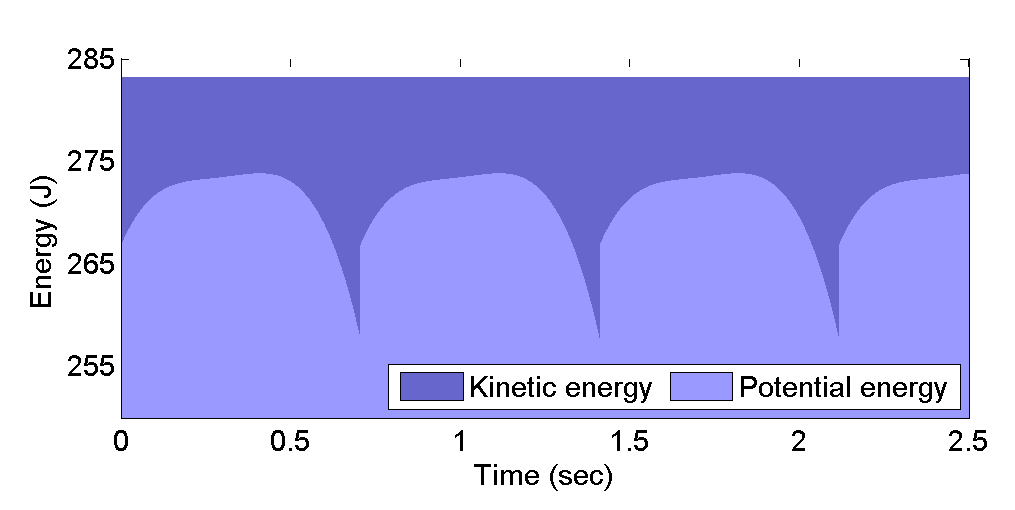
\includegraphics[width=1.0\columnwidth]{energy_cg2d_slope_model}
      \caption{Energy of the shaped system is conserved.}
    \end{figure}    
  }
  %  \only<3>{
  %    \includemedia[
  %      width=1.0\columnwidth,
  %      height=0.5625\columnwidth,
  %      addresource=amber2d.mp4,
  %      activate=pageopen,
  %      flashvars={source=amber2d.mp4&loop=true&autoPlay=true}
  %    ]{}{}%VPlayer9.swf}
  %  }

  \only<3>{
    Energy shaping can be achieved using:
    \begin{align*}
      \argmin_{u \in \Rn}  \, &\uu^{T} \uu\\
      \mbox{s.t. } & \Aclf\argsqdq \uu \leq \bclf\argsqdq
    \end{align*}
    where
    \begin{align*}
      \Aclf = 2 \eta \Lie{\xgbar} \eta, &&
      \bclf = -\resclfparam \eta^{2} - 2\eta \Lie{\xfbar} \eta,
    \end{align*}
    with
    \begin{align*}
      \eta = \Tnrg\argsqdq + \Unrg(\Psi\argsq) - \Eref.
    \end{align*}
  }

  \only<4>{
    \begin{figure}
      \centering
      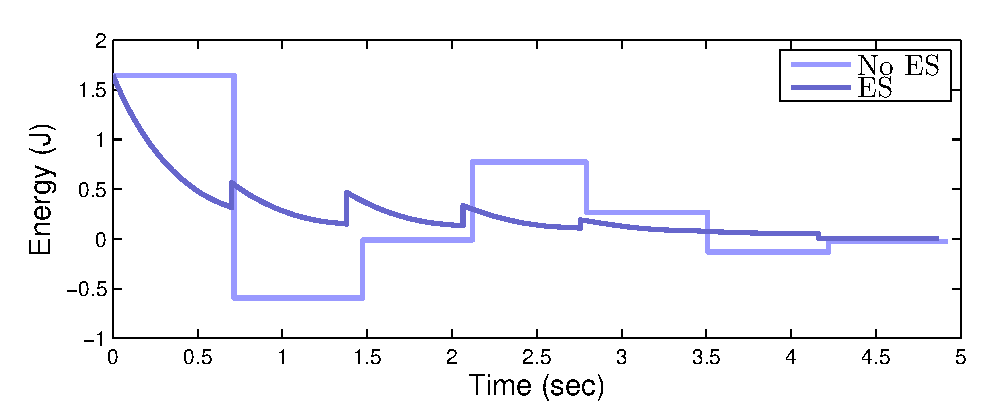
\includegraphics[width=1.0\columnwidth]{es_comparison_2link_conservative}
      \caption{Demonstration of energy shaping on 2-link biped.}
    \end{figure}
  }

  \only<5>{
    \begin{figure}
      \centering
      \includemedia[
        %width=1.0\columnwidth,
        %height=0.5625\columnwidth,
        width=1.0\columnwidth,
        height=0.5\columnwidth,
        addresource=cg2d_es.mp4,
        activate=pageopen,
        flashvars={source=cg2d_es.mp4&loop=true&autoPlay=true}
      ]{}{VPlayer9.swf}
      \caption{Energy shaping to stabilize to a gait from distant initial condition.}
    \end{figure}
  }

  \only<6> {
    \begin{figure}
      \centering
      \subfloat[Nominal system.]{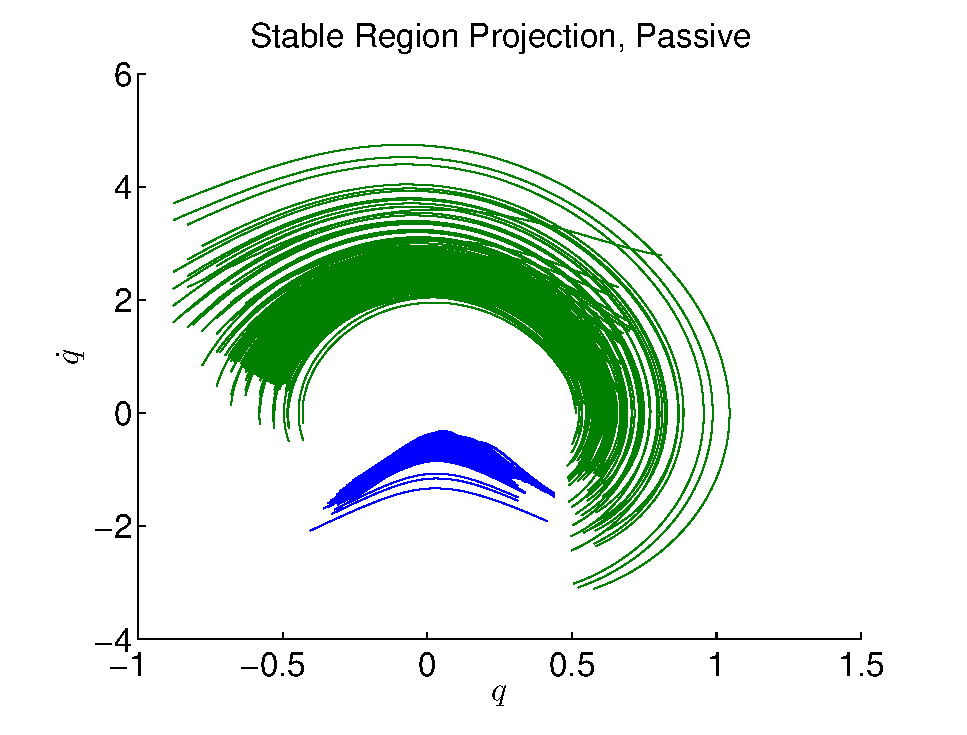
\includegraphics[width=.48\textwidth]{pp_eps_0}}
      \subfloat[Shaped system with $\resclfparam =
      \frac{1}{100}$.]{\includegraphics[width=.48\textwidth]{pp_eps_1_100}}
      \caption{Comparison of unshaped and shaped systems.}
    \end{figure}
  }

  \only<7> {
    \begin{figure}
      \centering
      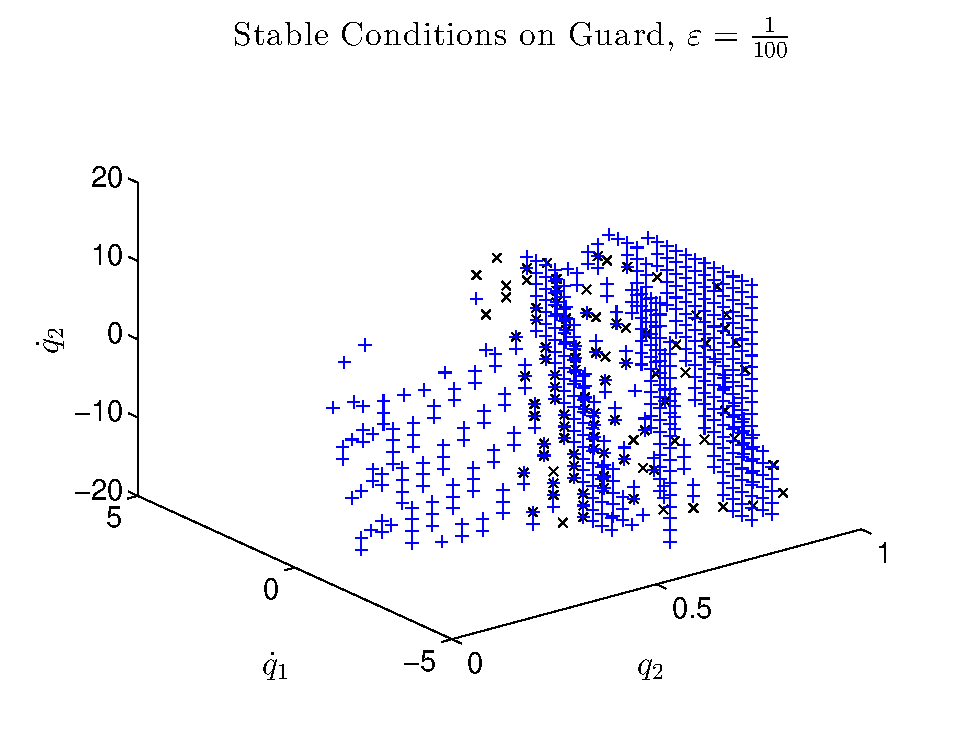
\includegraphics[height=.65\textheight]{poincare_cloud}
      \caption{A three-dimensional representation of the domain of attraction
        on the guard, comparing the unshaped and shaped system.}
    \end{figure}
  }
\end{frame}

\begin{frame}
  \frametitle{Example: 3-Link Biped}
  \only<1>{
    \begin{columns}
      \column{1.5in}
      Dynamic Model:
      \begin{align*}
        \M\argsq \ddq + \CG\argsqdq = \B\argsq \uu
      \end{align*}
      Control Law:
      \begin{align*}
        \vv\argsq& = \G\argsq - \G(\Psi\argsq)\\
        \vv_3\argsq& \ \  +\!= \ -\ck_{d} (\dot \vartheta_{T}^{a}\argsq)\\
        &\hspace{3.2em} -\ck_{p} (\vartheta_{T}^{a}\argsq - \vartheta_{T}^{d}\argsq)
      \end{align*}
      \column{1.5in}
      \begin{figure}
        \centering
        \def\svgwidth{1.0\columnwidth}
        \input{cg2d-3link-model.eps_latex}
        \vspace{-2em}
        \caption{3-link biped configuration.}
      \end{figure}
    \end{columns}
  }
  \only<2>{
    \begin{figure}
      \centering
      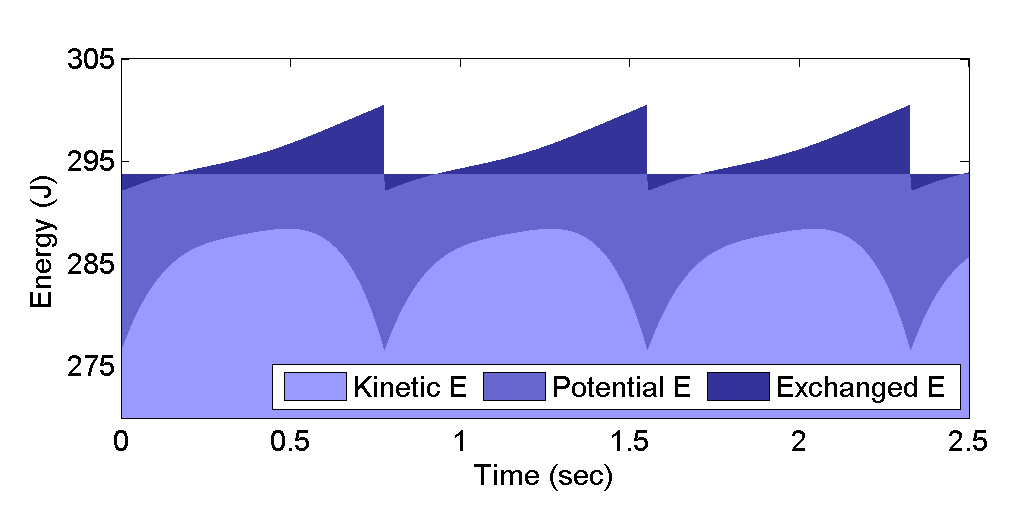
\includegraphics[width=1.0\columnwidth]{energy_conserved_cg2d_3link}
      \caption{The quantity $\Ec\argsqdqW = \Tnrg\argsqdq + \Unrg\argsq -
        \int_{0}^{t} \wrench_{\nc} \cdot \frac{d\q}{d\tau} d\tau$ is
        conserved.}
    \end{figure}
  }
  \only<3>{
    \begin{figure}
      \centering
      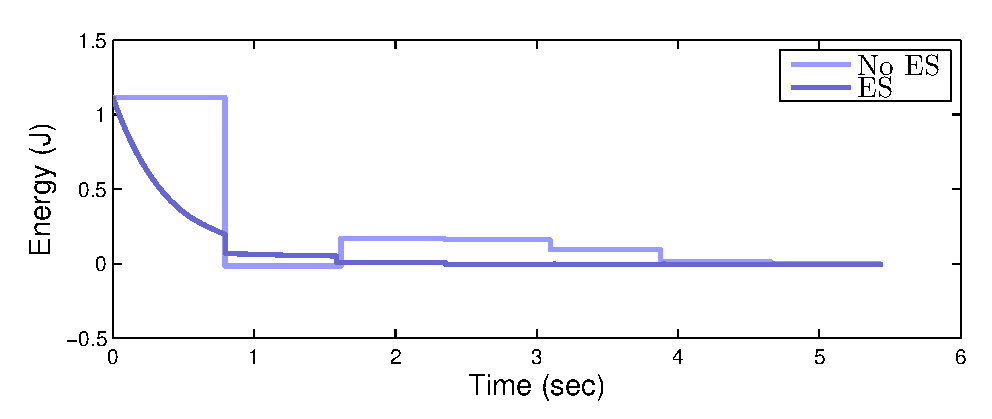
\includegraphics[width=1.0\columnwidth]{es_comparison_3link}
      \caption{Demonstration of energy shaping on 3-link biped.}
    \end{figure}
  }


  \only<4>{
    \begin{figure}
      \centering
      \includemedia[
        %width=1.0\columnwidth,
        %height=0.5625\columnwidth,
        width=1.0\columnwidth,
        height=0.5\columnwidth,
        addresource=3link_es.mp4,
        activate=pageopen,
        flashvars={source=3link_es.mp4&loop=true&autoPlay=true}
      ]{}{VPlayer9.swf}
      \caption{Energy shaping to stabilize to a gait from distant initial condition.}
    \end{figure}
  }

\end{frame}

\begin{frame}
  \frametitle{Multi-Domain Hybrid Systems}
  \begin{itemize}
  \item Complex hybrid systems are made by stitching together domains.
  \item Conserved energy is unique to each domain, i.e.,
    \begin{align*}
      \Ez^{1} \to \Ez^{2} \to \cdots \to \Ez^{n-1} \to \Ez^{n} \to \Ez^{1} \to \cdots
    \end{align*}
  \item Each domain shapes to a specific conserved energy level.
  \end{itemize}
\end{frame}


\begin{frame}
  \frametitle{Example: 7-Link Biped with Feet}
  \only<1>{
    %\blue{Appeared in {\bf Automatica}, Aug. 2014}
    \begin{columns}
      \column{1.5in}
      Dynamic Model:
      \begin{align*}
        \M\argsq \ddq + \CG\argsqdq = J^{T}\argsq \lambda + \B\argsq \uu
      \end{align*}
      \column{1.5in}
      \begin{figure}
        \centering
        \def\svgwidth{1.0\columnwidth}
        \vspace{-1em}
        \input{cg2d-7link-model.eps_latex}
        \vspace{-2em}
        \caption{7-link biped configuration.}
      \end{figure}
    \end{columns}
  }

  \only<2>{
    \begin{block}{Spring--Damper Controller}
      \begin{align*}
        \vv_{\mathit{SD}}\argsq = -\beta e^{-\rho \, h_{\nst}\argsq}
      \end{align*}
      where $\beta, \rho \in \Rpd$ and $h_{\nst} : \Q \to \R$ is the height of the Nonstance toe.
      Used on
      \begin{itemize}
      \item Stance ankle\\
      \item Nonstance ankle\\
      \item Absolute torso angle\\
      \item Non-stance knee spring (only in double support)
      \end{itemize}
      \blue{Provides passivity-based control and toe-off.}
    \end{block}
  }

  \only<3>{
    \begin{block}{Scuffing Prevention Controller}
      \begin{align*}
        \vv_{\mathit{SP}}\argsq = \ck_{p} \theta\argsq - \ck_{d} \dot \theta\argsqdq
      \end{align*}
      where $\ck_{p}, \ck_{d} \in \Rpd$. Used on
      \begin{itemize}
      \item Nonstance ankle
      \end{itemize}
      \blue{Prevents the nonstance toe from colliding with the ground prematurely.}
    \end{block}
  }

\only<4>{
  \begin{figure}
    \centering
      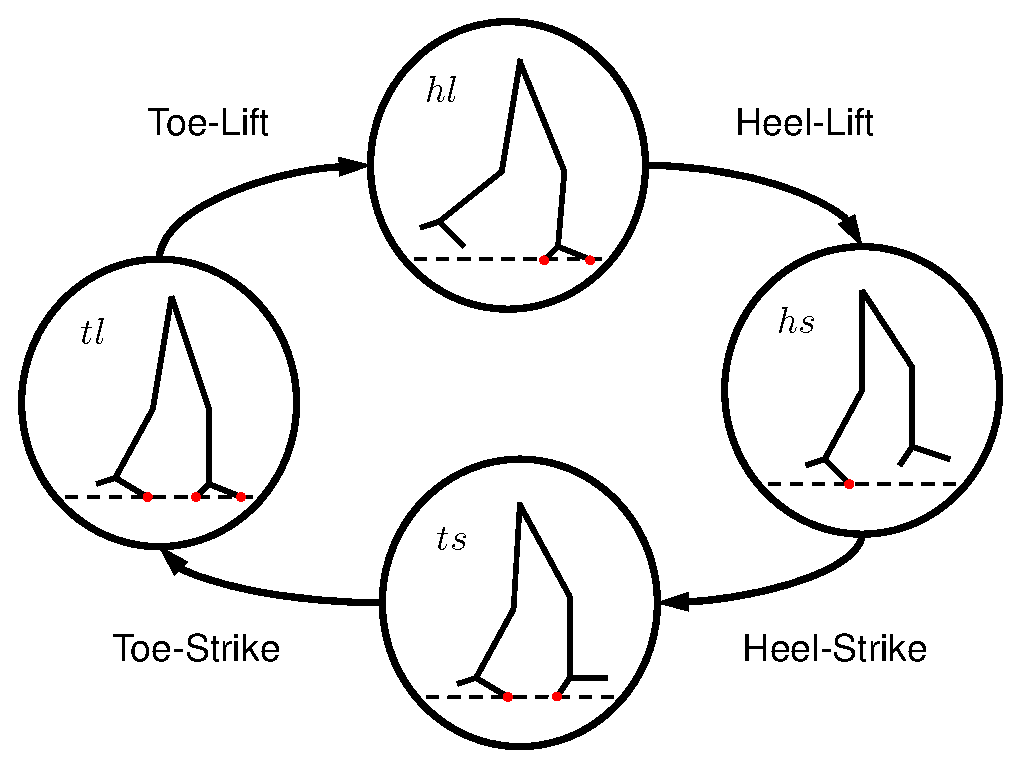
\includegraphics[height=.7\textheight]{domaingraph}
      \caption{The resulting gait traverses a four-domain directed graph.}
    \end{figure}
  }

  \only<5>{
    \begin{figure}
      \centering
      \includemedia[
        %width=1.0\columnwidth,
        %height=0.5625\columnwidth,
        width=1.0\columnwidth,
        height=0.5\columnwidth,
        addresource=7link_es.mp4,
        activate=pageopen,
        flashvars={source=7link_es.mp4&loop=true&autoPlay=true}
      ]{}{VPlayer9.swf}
      \caption{Energy shaping to stabilize to a gait.}
    \end{figure}
  }

  \only<6>{
    \begin{figure}
      \centering
      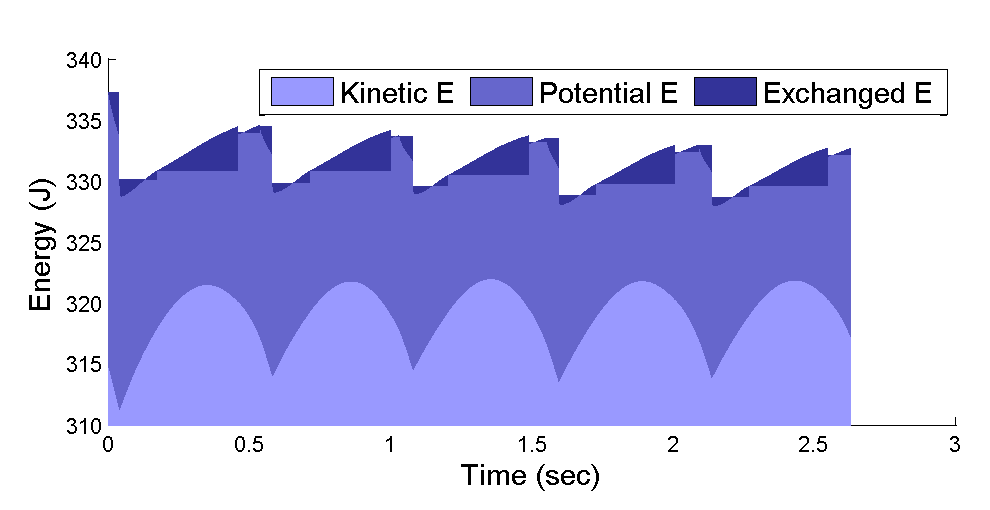
\includegraphics[width=1.0\columnwidth]{energy_conserved_7link}
      \caption{The quantity $\Ez \equiv \Tnrg\argsqdq + \Unrg\argsq -
        \int_{0}^{t} \wrench_{\nc} \cdot \frac{d\q}{d\tau} d\tau$ is
        conserved.}
    \end{figure}
  }

  \only<7>{
    \begin{figure}
      \centering
      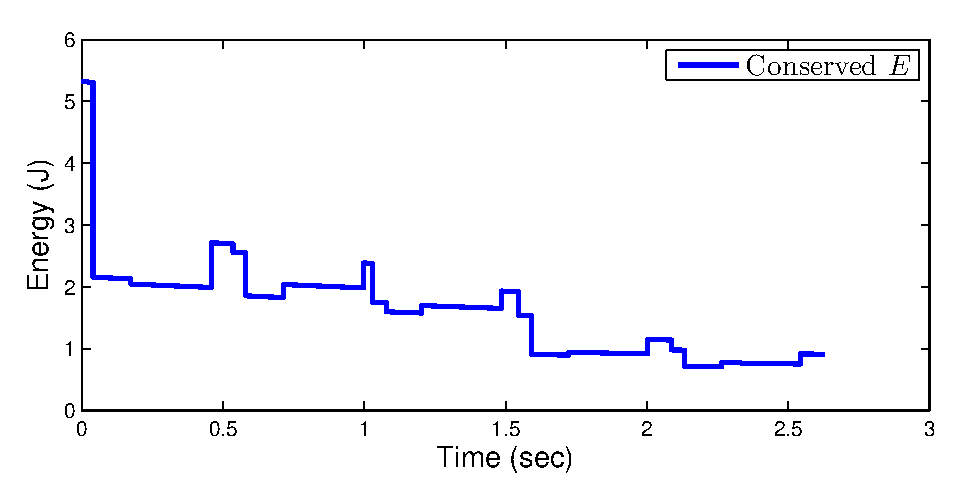
\includegraphics[width=1.0\columnwidth]{energy_conserved_7link_outline}
      \caption{The quantity $\Ez \equiv \Tnrg\argsqdq + \Unrg\argsq -
        \int_{t_0}^{t} \wrench_{\nc} \cdot \frac{d\q}{d\tau} d\tau$ is
        conserved.}
    \end{figure}
  }
  \only<8>{
    \begin{figure}
      \centering
      \includemedia[
        %width=1.0\columnwidth,
        %height=0.5625\columnwidth,
        width=1.0\columnwidth,
        height=0.5\columnwidth,
        addresource=7link_noes.mp4,
        activate=pageopen,
        flashvars={source=7link_noes.mp4&loop=true&autoPlay=true}
      ]{}{VPlayer9.swf}
      \caption{Many steps on the limit cycle.}
    \end{figure}
  }
\end{frame}
